\chapter{Plan y resultados de pruebas}

\section{Principio de verificación}

Cada prueba define precondición, acción, resultado esperado y evidencia. Esta estructura impide confundir una intención de diseño con un resultado observado. Las pruebas locales se ejecutaron sobre los archivos versionados. La evidencia del 22 de octubre de 2026 demuestra también el despliegue en AWS y las dos pruebas de conectividad. Los cinco controles definidos para el alcance de la Fase 1 están verificados.

\section{Prueba P-01: capacidad y no solapamiento}

\textbf{Precondición:} Python 3 disponible.

\textbf{Acción:} ejecutar \code{python scripts/validate-network.py}.

\textbf{Criterios:} todas las subredes deben pertenecer al \code{/24}; ninguna puede superponerse; $2^{32-p}-5$ debe cubrir la demanda; el bloque de reserva no debe intersectar una subred activa.

\textbf{Resultado:} \statusok. La suma de bloques es 256, todos los comienzos son canónicos y cada capacidad supera la demanda declarada. La salida completa se conserva como texto UTF-8.

\section{Prueba P-02: formato y validez de Terraform}

\textbf{Precondición:} Terraform y el proveedor oficial de AWS inicializados.

\textbf{Acción:} ejecutar \code{terraform fmt -check -recursive} y \code{terraform validate -no-color}.

\textbf{Criterio:} el formateador no propone cambios y la validación finaliza con código cero.

\textbf{Resultado:} \statusok. La salida registrada indica: ``Success! The configuration is valid.''

\begin{figure}[H]
\centering
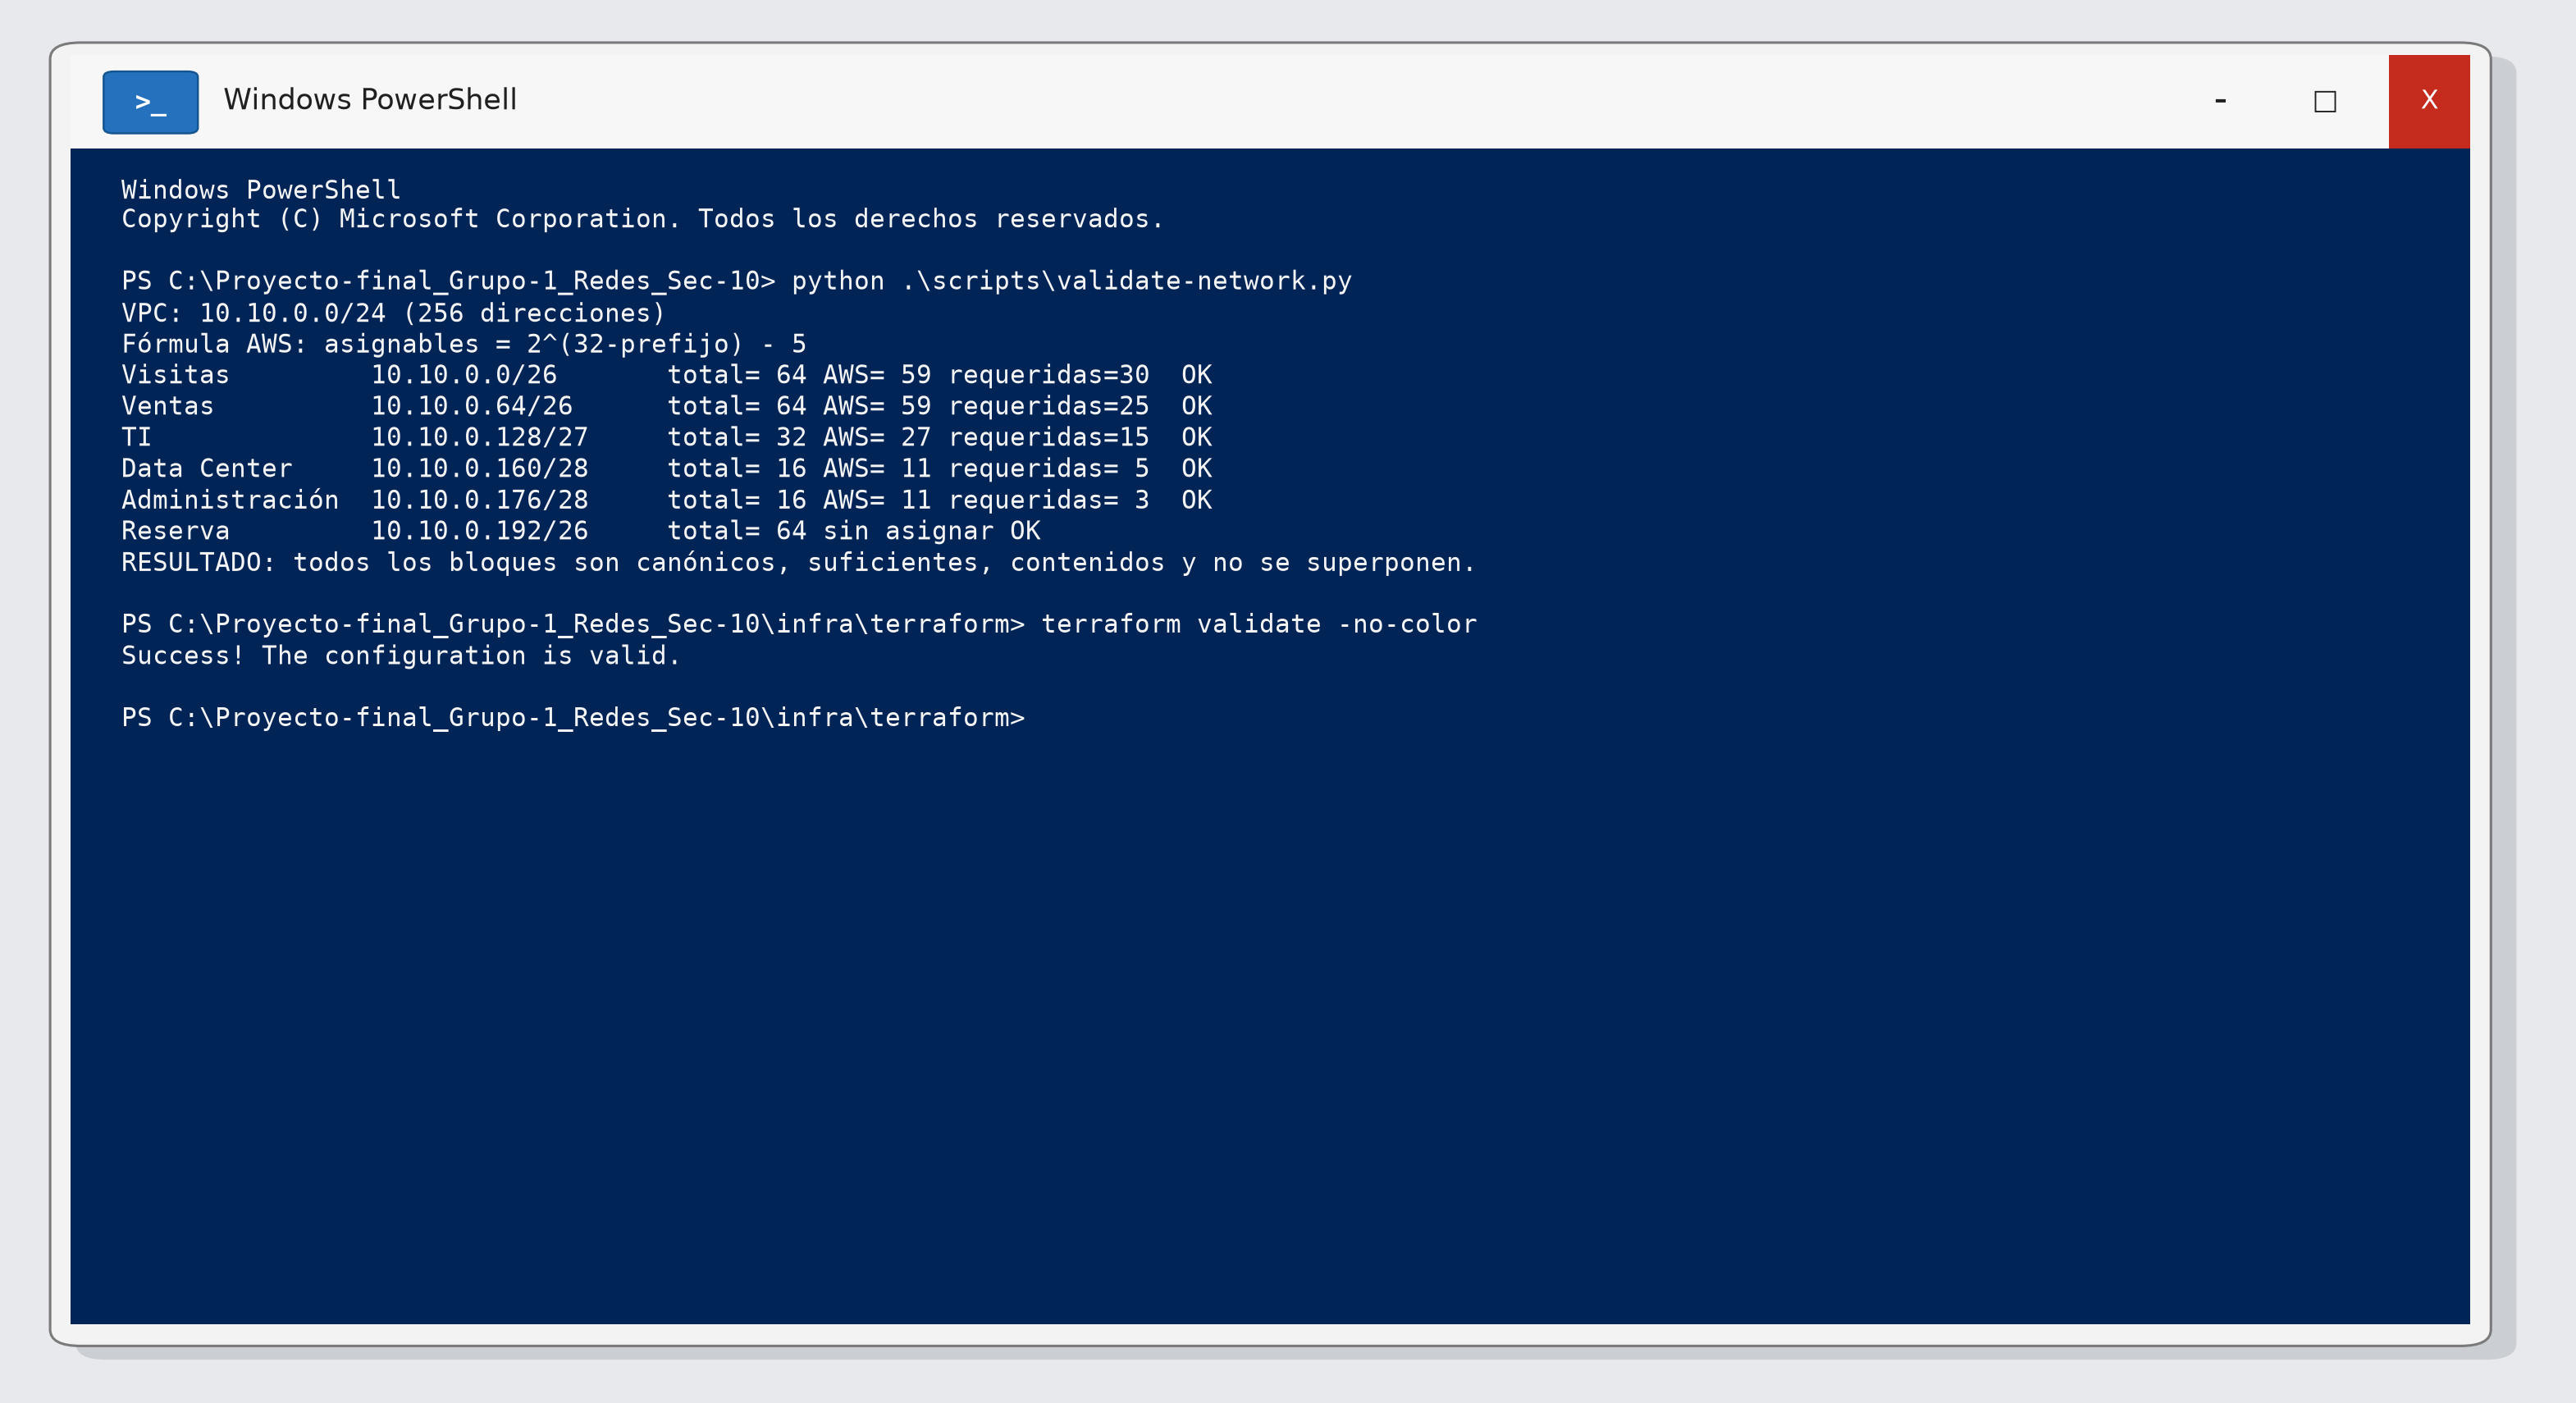
\includegraphics[width=0.93\textwidth]{validacion-local.png}
\caption{Captura reproducible de las validaciones locales.}
\label{fig:local-validation}
\end{figure}

\section{Prueba P-03: planificación contra el proveedor}

\textbf{Precondición:} credenciales AWS configuradas mediante un mecanismo admitido por el proveedor.

\textbf{Acción:} ejecutar \code{terraform plan} primero con cómputo deshabilitado y luego con las variables de prueba.

\textbf{Criterio:} el plan reconoce la identidad, consulta zona y AMI, y propone exclusivamente los recursos documentados.

\textbf{Resultado actual:} \statusok. La identidad AWS fue reconocida, la región se confirmó como \code{us-east-1} y Terraform produjo un plan compuesto únicamente por altas previstas. La Figura~\ref{fig:terraform-cloud-plan} muestra recursos para la VPC, cinco subredes, tablas y asociaciones de rutas, grupos de seguridad, llave temporal, bastión y dos instancias de Ventas.

\begin{figure}[H]
\centering
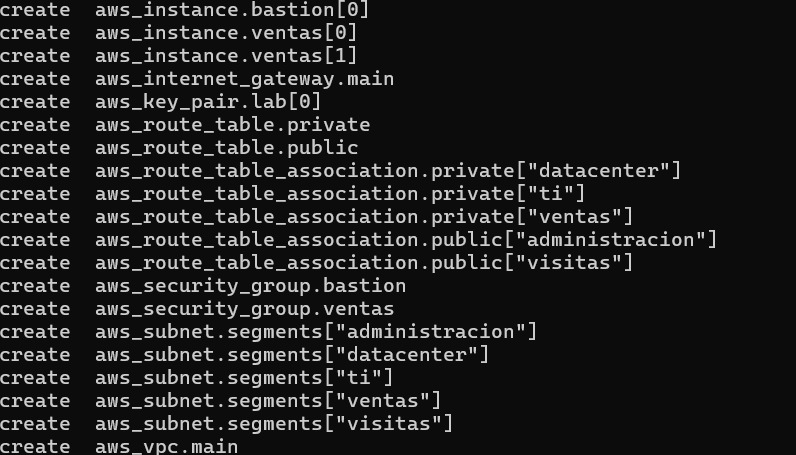
\includegraphics[width=0.96\textwidth]{terraform-plan-recursos-previstos.jpeg}
\caption{Evidencia genuina del plan Terraform contra AWS. Esta captura documenta la revisión previa al \code{apply}; la ejecución real se acredita por separado.}
\label{fig:terraform-cloud-plan}
\end{figure}

Esta prueba verifica autenticación y planificación contra el proveedor. La existencia posterior de la infraestructura no se infiere del plan: se demuestra mediante la salida real de \code{terraform apply}, los identificadores observados y las capturas de la Figura~\ref{fig:aws-deployment-real}.

\section{Prueba P-04: conectividad privada}

\textbf{Precondición:} bastión y dos instancias de Ventas en estado \emph{running}; llaves y reglas activas.

\textbf{Acción:} desde la instancia Ventas A ejecutar:

\begin{Verbatim}[fontsize=\small,frame=single]
ping -c 4 <IP_PRIVADA_VENTAS_B>
\end{Verbatim}

El script \code{scripts/test-connectivity.ps1} utiliza SSH con salto por el bastión, registra origen, destino, fecha y salida, y guarda \code{evidence/connectivity/ping-private.txt}.

\textbf{Criterio:} cuatro paquetes transmitidos, cuatro recibidos y 0\% de pérdida. Las dos direcciones deben pertenecer a \code{10.10.0.64/26}; ninguna debe ser pública.

\textbf{Resultado:} \statusok. Desde \code{10.10.0.71} se enviaron cuatro paquetes a \code{10.10.0.79}; se recibieron los cuatro y se observó 0\% de pérdida. Ambas direcciones pertenecen a la subred de Ventas \code{10.10.0.64/26}. El siguiente extracto proviene del registro genuino conservado en el repositorio:

\VerbatimInput[fontsize=\footnotesize,frame=single,firstline=7,lastline=15]{../../evidence/connectivity/ping-private.txt}

\section{Prueba P-05: aislamiento}

Después del ping exitoso, se intenta ICMP desde el bastión hacia una instancia de Ventas. La regla de Ventas acepta ICMP sólo desde su propio grupo, por lo que el tráfico del bastión debe fallar. Esta prueba negativa demuestra que permitir administración SSH no equivale a permitir todo protocolo.

\textbf{Resultado:} \statusok. El bastión intentó alcanzar \code{10.10.0.71}; se transmitieron cuatro paquetes, ninguno fue recibido y la pérdida fue 100\%. El resultado es coherente con la regla que acepta ICMP sólo entre miembros del grupo de Ventas.

\begin{figure}[H]
\centering
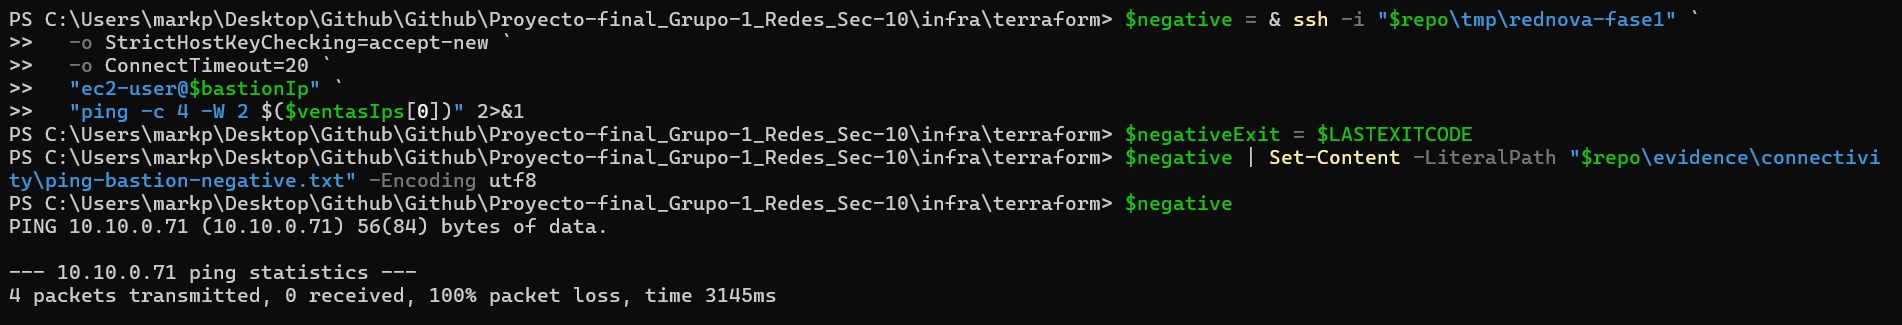
\includegraphics[width=0.94\textwidth]{04-prueba-icmp-bastion-bloqueada.png}
\caption{Prueba genuina de aislamiento: ICMP desde el bastión hacia Ventas fue bloqueado.}
\label{fig:bastion-negative-test}
\end{figure}

\section{Matriz de resultados}

\begin{table}[H]
\centering
\caption{Resumen de verificación}
\begin{tabularx}{\textwidth}{p{1.6cm}Y p{3.4cm}}
\toprule
\textbf{Prueba} & \textbf{Propiedad observada} & \textbf{Estado} \\
\midrule
P-01 & Capacidad, contención, canonicidad y no solapamiento. & \statusok \\
P-02 & Sintaxis, formato y relaciones del código Terraform. & \statusok \\
P-03 & Resolución de recursos mediante una identidad AWS. & \statusok \\
P-04 & Conectividad ICMP privada dentro de Ventas. & \statusok \\
P-05 & Rechazo ICMP desde el bastión. & \statusok \\
\bottomrule
\end{tabularx}
\end{table}

\section{Interpretación}

Los resultados locales confirman que el diseño es internamente consistente y que Terraform puede interpretarlo. La evidencia externa confirma una identidad activa, la región, el plan, la creación de 20 recursos, la conectividad privada y el aislamiento del bastión. Esa cadena conserva la distinción entre intención y observación: el \code{plan} no sustituye el \code{apply}, y el \code{apply} no sustituye las pruebas de tráfico. Las cinco pruebas definidas para el alcance de la Fase 1 están verificadas.
